\section{Les données à notre disposition}

Les données du problème concernent les contentrations de trois types de polluants ($NO_2$, $PM_{10}$, $PM_{2,5}$) sur une période de temps T donnée dans six villes inconnues, numérotées de 0 à 5.
Chaque ville comporte 4 ou 5 stations (29 au total sur les six villes, numérotées de 1 à 29).

\subsection{Variables explicatives}

Pour chacune des stations, nous avons les variables explicatives suivantes:
\begin{itemize}
  \item 18 variables statiques, qui nous renseignent sur l'entourage du point où les mesures sont faites:
  \begin{itemize}
    \item la surface cumulée de zones résidentielles à faible densité dans un rayon de 25/50/150/250/500 mètres autour du point
    \item la surface cumulée de zones résidentielles à haute densité dans un rayon de 25/50/150/250/500 mètres autour du point
    \item la surface cumulée de zones industrielles dans un rayon de 500 mètres autour du point
    \item la surface cumulée de zones portuaires dans un rayon de 2500 mètres autour du point
    \item la surface cumulée d'espaces verts dans un rayon de 2500 mètres autour du point
    \item la distance cumulée de routes dans un rayon de 50/150/250/500 mètres autour du point
    \item l'inverse de la distance à la route la plus proche
  \end{itemize}
  \item 9 variables dynamiques, dont on a les valeurs sur pratiquement toute la periode T, à intervalles de temps d'une heure:
  \begin{itemize}
    \item La température
    \item La vitesse du vent
    \item l'orientation du vent, via la valeur du cosinus et du sinus de l'angle par rapport à une référence inconnue
    \item l'ennuagement
    \item l'intensité des précipitations
    \item la probabilité de précipitations
    \item la pression
    \item une variable booléenne qui indique si le jour est calme ou non
  \end{itemize}
\end{itemize}

\subsection{Données d'entrainement}

Comme données d'entrainement, nous avons les concentrations en polluants à intervalle de temps d'une heure sur toute la période pour 2 ou 3 stations par ville (17 sur 29 au total).
Pour les 12 autre stations (2 par ville), nous n'avons \textbf{aucune} valeur de concentration en polluants.

\subsection{Problème posé}

Le but est de prédire la concentration en polluant sur ces 12 stations sur sur tout la période T donnée.

Le problème est donc un problème de régression très général : étant données les variables explicatives et l'évolution temporelle des concentration en polluants à certain points sur une période T, prédire l'évolution temporelle des concentration en d'autre points à partir des données météorologiques et statiques.
Pour ce faire, nous n'avons que très peu d'exemples (2 ou 3 par ville), bien que la période T soit longue.
La tâche s'annonce donc compliquée.

\subsection{Remarques sur les données}
Quelques remarques sur les données:
\begin{itemize}
  \item
    Le comportement physiques des trois polluants est très différent.
    Les particules $PM_{2,5}$ et $PM_{10}$ ont une taille entre 1 et 10 micromètres, pèsent ...
    Elle sont solubles dans l'eau; la pluie a donc une très grande influence sur leur concentration dans l'air.
    Le $NO_2$ est une molécule de taille ..., beaucoup plus petite que les particules, avec une inertie beaucoup plus faible.
    Elle est de plus bien moins sensible à la pluie que les micro particules.
    Le comportement des différents pollutants est donc radicalement différent.
    Cela suggère de traiter différemment les microparticules et le $NO_2$.
  \item
    Nous n'avons aucune donnée géographique qui nous renseigne sur la position relative des différents points les uns par rapport aux autre, ni sur la position relative des éléments (par exemples les routes) qui sont dans l'entourage du point auquel est fait la mesure.
    Nous ne pouvons donc pas espérer avoir de résultats précis.
    Prenons par exemple la carte de pollution en $NO_2$ de la ville Gothenburg qui est prise en exemple dans l'article \cite{}:
    \begin{center}
    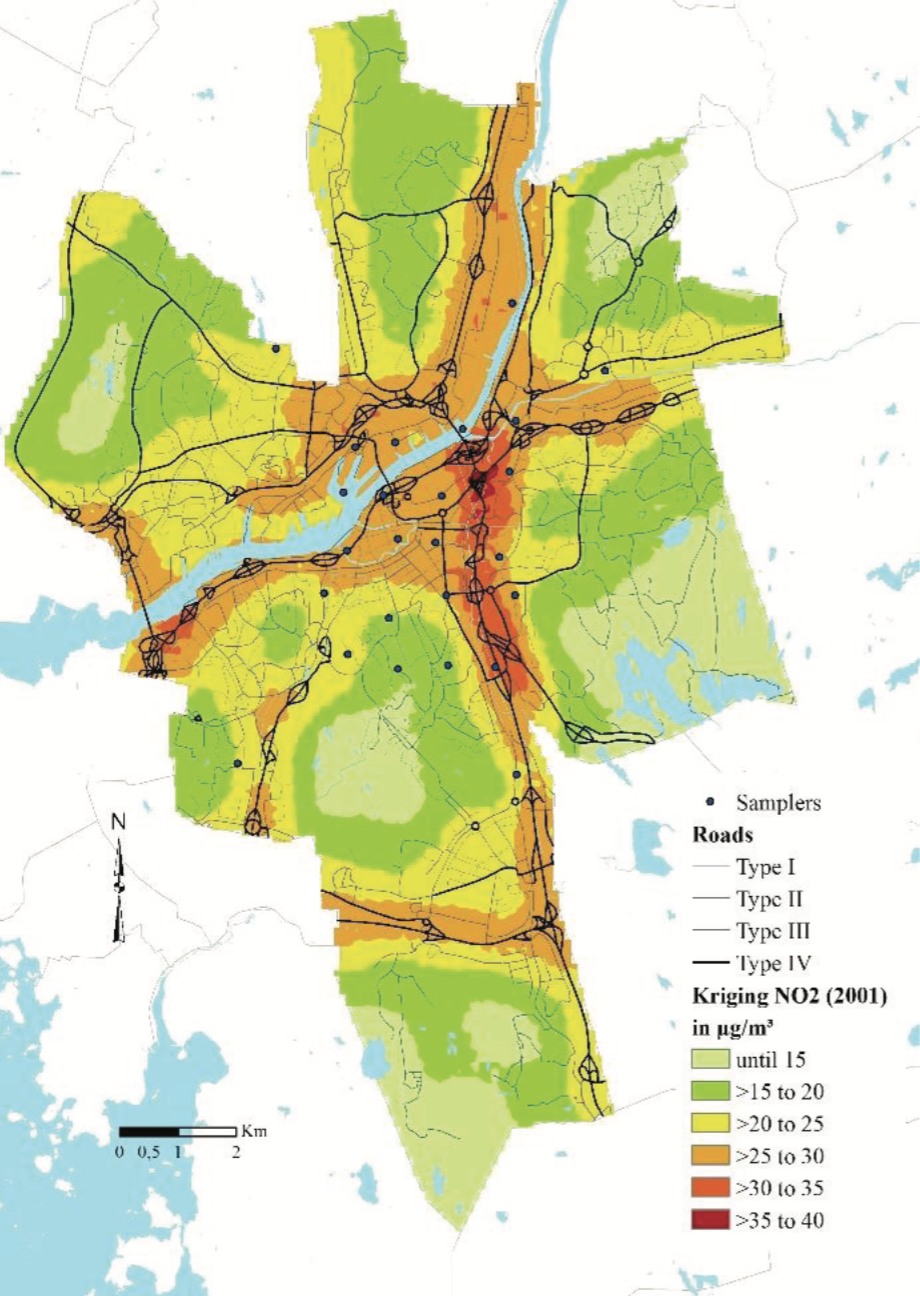
\includegraphics[height=8cm]{images/pollution_gothenburg.png}
    \end{center}
    On constate que la pollution en $NO_2$ est phénomène spatial, et on peut sans aucun doute trouver des points qui auront les même valeurs statiques (surfaces cumulées) et pour lesquels le niveau de pollution est pourtant très différent.
    Notons au passage que les routes sont classés selon différents types qui semblent être déterminants pour la pollution en $NO_2$, or nous n'avons qu'un type de route à notre disposition
  \item
    A une heure donnée, les données météorologique (température, vent, pression, ennuagement) sont les mêmes pour toutes les stations d'une zone.
    Ce sont donc uniquement les données statiques qui différencient les stations les unes des autres.
  \item
    L'angle d'orientation du vent nous est donnée par son cosinus et son sinus, dont la somme des carrés ne font pas 1 en général (moyenne = 0.995, écart type =  0.06 , maximum =  1.995 , minimum = 2.4 $\cdot 10^{-11}$)
  \item
    Les données statiques nous sytématiquement répétées pour chaque valeur temporelle d'un polluant.
    Nous avons donc fait un script pour vérifier que ce sont effectivement toujours les mêmes pour une station donnée.
\end{itemize}

